% fig_harm_filter_pipeline.tex
% Block diagram: harmonic pre-filter in the SAMBP 87L processing chain (TR-21)
% Shows new harmonic LS estimator stage inserted before the LM estimator
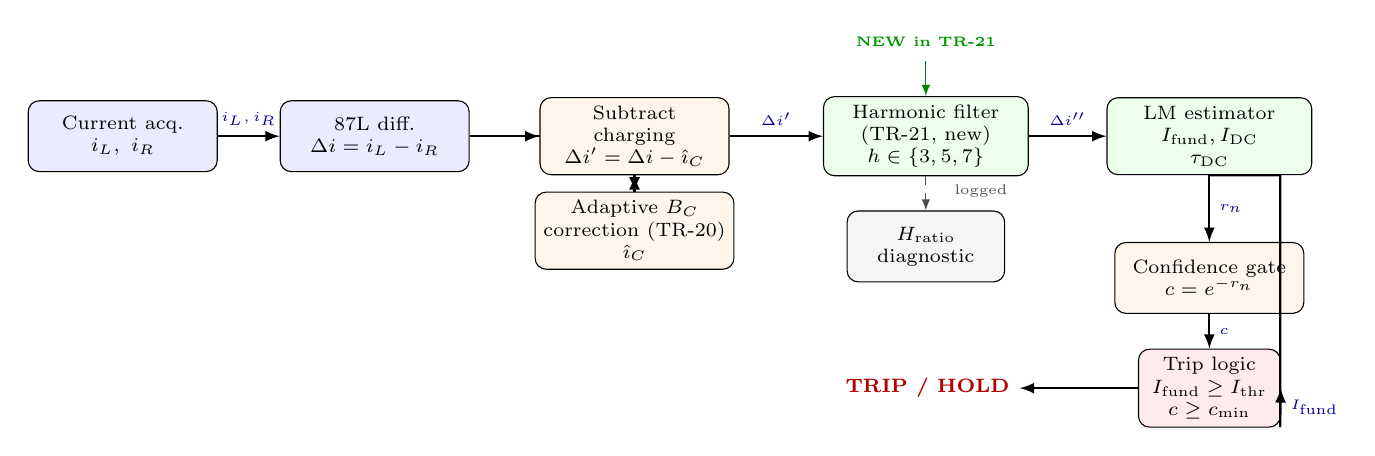
\begin{tikzpicture}[
  blk/.style={draw, rounded corners=4pt, fill=blue!8,
              minimum width=2.4cm, minimum height=0.9cm,
              font=\scriptsize, align=center, inner sep=3pt},
  blk2/.style={draw, rounded corners=4pt, fill=green!8,
               minimum width=2.6cm, minimum height=0.9cm,
               font=\scriptsize, align=center, inner sep=3pt},
  blk3/.style={draw, rounded corners=4pt, fill=orange!8,
               minimum width=2.4cm, minimum height=0.9cm,
               font=\scriptsize, align=center, inner sep=3pt},
  blkr/.style={draw, rounded corners=4pt, fill=red!8,
               minimum width=1.8cm, minimum height=0.9cm,
               font=\scriptsize, align=center, inner sep=3pt},
  blkg/.style={draw, rounded corners=4pt, fill=gray!8,
               minimum width=2.0cm, minimum height=0.9cm,
               font=\scriptsize, align=center, inner sep=3pt},
  arr/.style={-latex, thick},
  sig/.style={font=\tiny\itshape, blue!60!black},
]

% ---- Stage 1: Measured differential ----------------------------------------
\node[blk] (acq) at (0, 0)
  {Current acq.\\$i_L,\ i_R$};

\node[blk] (diff) at (3.2, 0)
  {87L diff.\\$\Delta i = i_L - i_R$};
\draw[arr] (acq.east) -- node[above, sig]{$i_L, i_R$} (diff.west);

% ---- Stage 2: Charging correction (TR-15/TR-20) ----------------------------
\node[blk3] (charg) at (6.5, -1.2)
  {Adaptive $B_C$\\correction (TR-20)\\$\hat{\imath}_C$};
\draw[arr] (diff.east) -| node[right, sig, pos=0.4]{$\Delta i$} (charg.north);

\node[blk3] (sub1) at (6.5, 0)
  {Subtract\\charging\\$\Delta i' = \Delta i - \hat{\imath}_C$};
\draw[arr] (diff.east) -- (sub1.west);
\draw[arr] (charg.north) -- (sub1.south);

% ---- Stage 3 (NEW): Harmonic pre-filter ------------------------------------
\node[blk2] (hfilt) at (10.2, 0)
  {Harmonic filter\\(TR-21, new)\\$h \in \{3,5,7\}$};
\draw[arr] (sub1.east) -- node[above, sig]{$\Delta i'$} (hfilt.west);

\node[blkg] (hdiag) at (10.2, -1.4)
  {$H_{\rm ratio}$\\diagnostic};
\draw[-latex, gray!60!black, dashed]
  (hfilt.south) -- (hdiag.north);
\node[font=\tiny, gray!60!black] at (10.9, -0.7) {logged};

% ---- Stage 4: LM estimator -------------------------------------------------
\node[blk2] (lm) at (13.8, 0)
  {LM estimator\\$I_{\rm fund}, I_{\rm DC}$\\$\tau_{\rm DC}$};
\draw[arr] (hfilt.east) -- node[above, sig]{$\Delta i''$} (lm.west);

% ---- Stage 5: Confidence gate + Trip logic ---------------------------------
\node[blk3] (conf) at (13.8, -1.8)
  {Confidence gate\\$c = e^{-r_n}$};
\draw[arr] (lm.south) -- node[right, sig]{$r_n$} (conf.north);

\node[blkr] (trip) at (13.8, -3.2)
  {Trip logic\\$I_{\rm fund} \geq I_{\rm thr}$\\$c \geq c_{\min}$};
\draw[arr] (conf.south) -- node[right, sig]{$c$} (trip.north);
\draw[arr] (lm.south) -- ++(0.9, 0) -- ++(0, -3.2) -- (trip.east)
  node[midway, right, sig]{$I_{\rm fund}$};
\draw[arr] (trip.west) -- ++(-1.5, 0)
  node[left, font=\scriptsize\bfseries, red!70!black]{TRIP / HOLD};

% ---- "New in TR-21" label --------------------------------------------------
\node[font=\tiny\bfseries, green!60!black, align=center]
  at (10.2, 1.2) {NEW in TR-21};
\draw[-latex, green!50!black, thin]
  (10.2, 0.95) -- (hfilt.north);

\end{tikzpicture}
